
\documentclass[final]{beamer}

\usepackage[scale=1.24]{beamerposter} % Use the beamerposter package for laying out the poster

\usetheme{confposter} % Use the confposter theme supplied with this template

\setbeamercolor{block title}{fg=ngreen,bg=white} % Colors of the block titles
\setbeamercolor{block body}{fg=black,bg=white} % Colors of the body of blocks
\setbeamercolor{block alerted title}{fg=white,bg=dblue!70} % Colors of the highlighted block titles
\setbeamercolor{block alerted body}{fg=black,bg=dblue!10} % Colors of the body of highlighted blocks
% Many more colors are available for use in beamerthemeconfposter.sty

%-----------------------------------------------------------
% Define the column widths and overall poster size
% To set effective sepwid, onecolwid and twocolwid values, first choose how many columns you want and how much separation you want between columns
% In this template, the separation width chosen is 0.024 of the paper width and a 4-column layout
% onecolwid should therefore be (1-(# of columns+1)*sepwid)/# of columns e.g. (1-(4+1)*0.024)/4 = 0.22
% Set twocolwid to be (2*onecolwid)+sepwid = 0.464
% Set threecolwid to be (3*onecolwid)+2*sepwid = 0.708

\newlength{\sepwid}
\newlength{\onecolwid}
\newlength{\twocolwid}
\newlength{\threecolwid}
\setlength{\paperwidth}{48in} % A0 width: 46.8in
\setlength{\paperheight}{36in} % A0 height: 33.1in
\setlength{\sepwid}{0.024\paperwidth} % Separation width (white space) between columns
\setlength{\onecolwid}{0.22\paperwidth} % Width of one column
\setlength{\twocolwid}{0.464\paperwidth} % Width of two columns
\setlength{\threecolwid}{0.708\paperwidth} % Width of three columns
\setlength{\topmargin}{-0.5in} % Reduce the top margin size
%-----------------------------------------------------------

\usepackage{graphicx}  % Required for including images

\usepackage{booktabs} % Top and bottom rules for tables

%----------------------------------------------------------------------------------------
%	TITLE SECTION 
%----------------------------------------------------------------------------------------

\title{Plankton Barbecue} % Poster title

\author{Juan D. Chacon} % Author(s)

\institute{Simon Fraser University Spring 2019} % Institution(s)

%----------------------------------------------------------------------------------------

\begin{document}

\addtobeamertemplate{block end}{}{\vspace*{2ex}} % White space under blocks
\addtobeamertemplate{block alerted end}{}{\vspace*{2ex}} % White space under highlighted (alert) blocks

\setlength{\belowcaptionskip}{2ex} % White space under figures
\setlength\belowdisplayshortskip{2ex} % White space under equations

\begin{frame}[t] % The whole poster is enclosed in one beamer frame

\begin{columns}[t] % The whole poster consists of three major columns, the second of which is split into two columns twice - the [t] option aligns each column's content to the top

\begin{column}{\sepwid}\end{column} % Empty spacer column

\begin{column}{\onecolwid} % The first column

%------------------------------------------------
%	Planton Picture
%------------------------------------------------
\begin{figure}

\includegraphics[width=0.45\linewidth]{images/planktonBBQRCropped.pdf}
\end{figure}

%----------------------------------------------------------------------------------------
%	Introduction
%----------------------------------------------------------------------------------------

\begin{block}{Introduction}

\textbf{Natural Thermal Convection}

Those plumes comming out from our BBQ grill are caused by differences on density consequence of temperature variations.
\vspace{1em}
\begin{alertblock}{Governing Equations}
\begin{itemize}
\item \textbf{($\approx$) Momentum:}
$$\frac{\partial\omega}{\partial t}+\frac{\partial\psi}{\partial y}\frac{\partial\omega}{\partial x}-\frac{\partial\psi}{\partial x}\frac{\partial\omega}{\partial y}=\frac{1}{Re}\nabla^{2}\omega+\beta g\frac{\partial T}{\partial x}$$
\item \textbf{Stream fnc - Vorticity - Velocity:}
$$\nabla^{2}\psi=-\omega,\:\: u=\frac{\partial\psi}{\partial y},\:\: v=-\frac{\partial\psi}{\partial x}$$
\item \textbf{Energy:}
$$\frac{\partial T}{\partial t}+\left(\overrightarrow{u}\cdot\nabla T\right)=\frac{1}{RePr}\nabla^{2}T$$
\item \textbf{(Bonus!!!) Mass Transfer:}
$$\frac{\partial c}{\partial t}+\left(\overrightarrow{u}\cdot\nabla c\right)=\frac{1}{Pe}\nabla^{2}c$$
\end{itemize}
\end{alertblock}
Where the last Eq. models a substance moving with the fluid.
\end{block}

%----------------------------------------------------------------------------------------
%	METHOD
%----------------------------------------------------------------------------------------
\vspace{-1em}
\begin{block}{Method}
To solve numerically the equations ...
\begin{enumerate}
\item Set up the initial conditions for $\psi$, $u$ and $v$.
\item Solve the vorticity equation. (Exp FTCS).
\item Solve the Poisson equation for $\psi$. (Std. discr. $\nabla^{2}$).
\item Compute the new velocity from $\psi$.
\item Solve the energy equation for $T$. (Exp FTCS).
\item Solve the mass transfer equation. (Exp FTCS).
\item Go to step 2.
\end{enumerate}
\end{block}

\end{column} % End of the first column

\begin{column}{\sepwid}\end{column} % Empty spacer column

\begin{column}{\twocolwid} % Begin a column which is two columns wide (column 2)

\begin{columns}[t,totalwidth=\twocolwid] % Split up the two columns wide column

\begin{column}{\onecolwid}\vspace{-.6in} % The first column within column 2 (column 2.1)

%----------------------------------------------------------------------------------------
%	COL2
%----------------------------------------------------------------------------------------

\begin{block}{BBQ Grill: Air Thermal Convection}
	As benchmark parameters we chose:
	$$Re=4365.30, \: Pr=0.72, \: Pe=0.07$$
	For a rectangular cavity width dimensions: 0.65m height, 2.6m wide, and normalized temperatures $Tc=292.5^{\circ}K$, $Th=293.5^{\circ}K$.

	\vspace{1em}
	The Figure 2 shows the normalized velocities, temperature and concentration evolution for several times, some remarkable facts are:
	\begin{itemize}
		\item Buoyancy force makes rise the warmer water from the bottom.
		\item There are cell formations even for early times.
		\item Iso-thermal and Iso-concetration regions.
	\end{itemize}
\end{block}

%----------------------------------------------------------------------------------------

\end{column} % End of column 2.1

\begin{column}{\onecolwid}\vspace{-.6in} % The second column within column 2 (column 2.2)

%----------------------------------------------------------------------------------------
%	Cells and Spatial Dependency
%----------------------------------------------------------------------------------------

\begin{block}{Cells and Spatial Resolution}
	The Figure 1 shows that the simulation results depend on the discretization size. In the coarser discretization only 4 cells Rayleigh-Benard cells form, compared to 6 in the finer one. This indicates that some discretizations cannot completely resolve the structure of the flow.
	\vspace{1em}
\begin{figure}
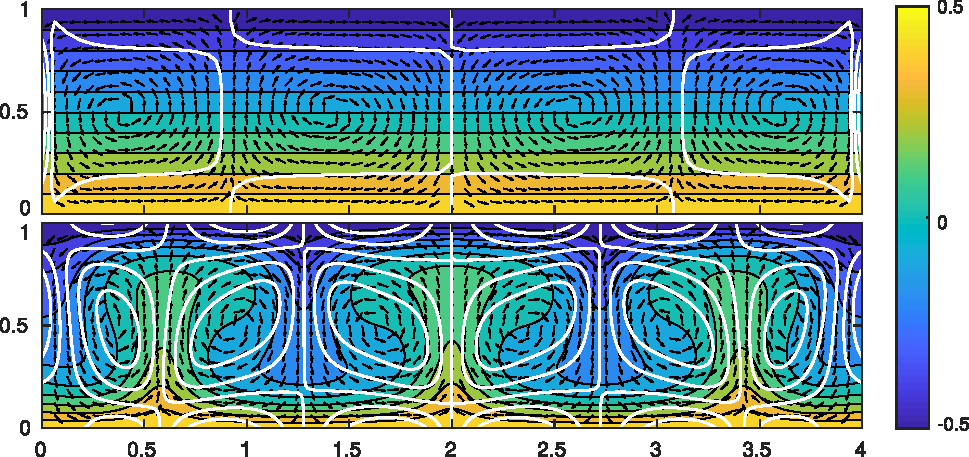
\includegraphics[width=1.0\linewidth]{images/cells.pdf}
	\caption{\hspace{1em}Cells on grids: (top) $\Delta x=156\times10^{-3}, \Delta y=62.5\times10^{-3}$ (bottom) $\Delta x=39\times10^{-3}, \Delta y=15.4\times10^{-3}.$}
\end{figure}
\end{block}

%----------------------------------------------------------------------------------------

\end{column} % End of column 2.2

\end{columns} % End of the split of column 2 - any content after this will now take up 2 columns width

%----------------------------------------------------------------------------------------
%	IMPORTANT To REMEMBER
%----------------------------------------------------------------------------------------
\vspace{-2em}
\begin{figure}
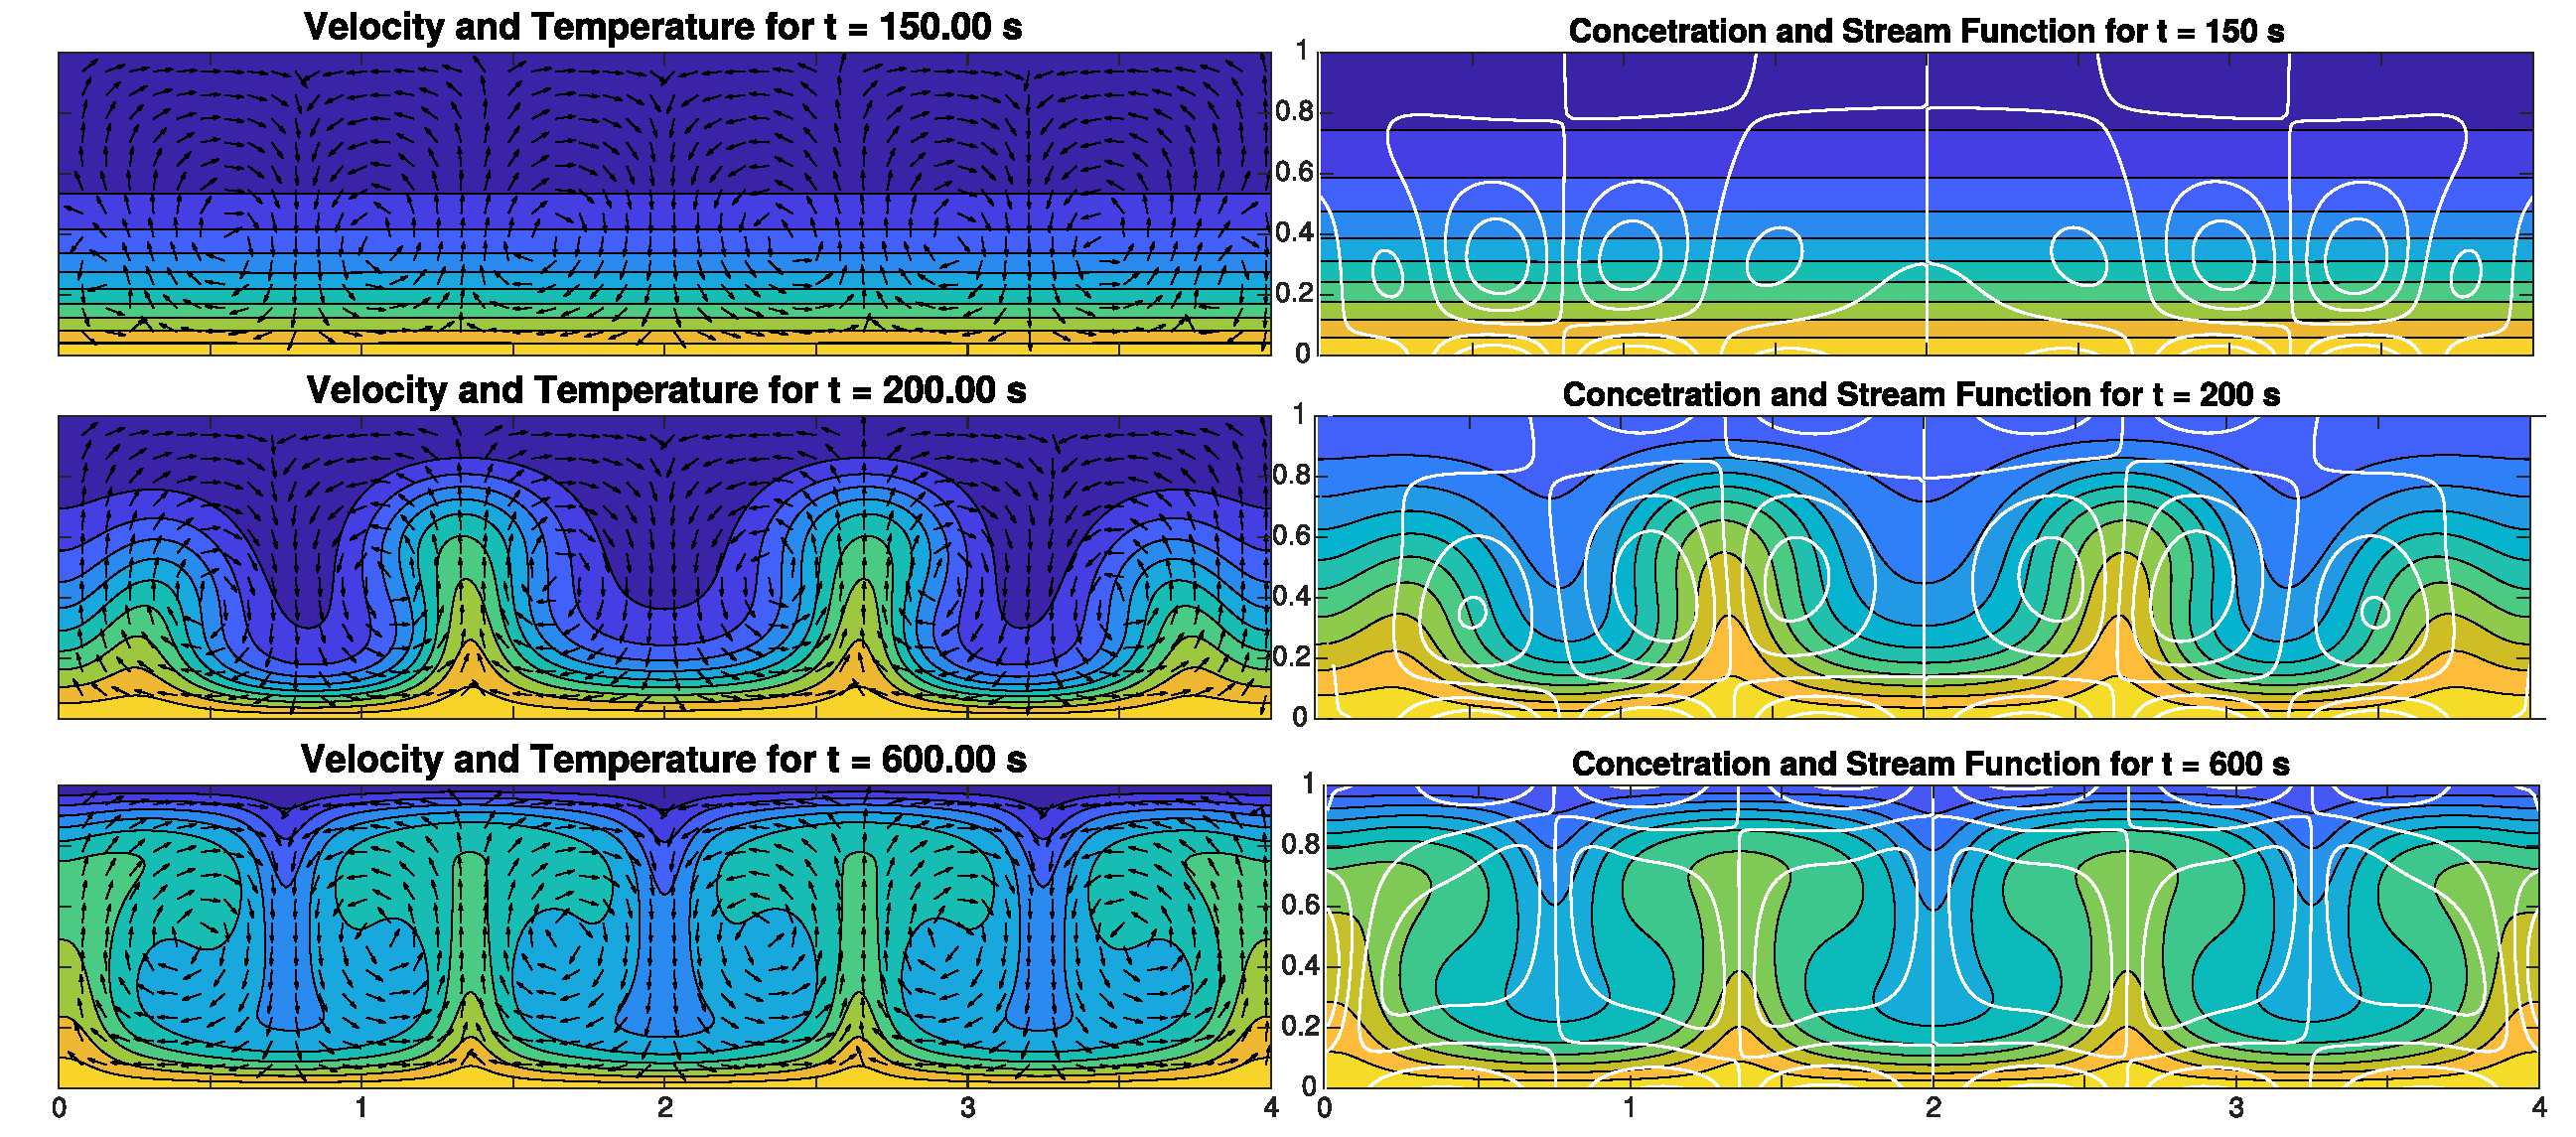
\includegraphics[width=1.0\linewidth]{images/figure1.pdf}
\caption{Air thermal convection and mass transfer normalized velocity, temperature and mass concentration for different times.}
\end{figure}

\begin{block}{Numerical Convergence}
	\begin{columns}[t,totalwidth=\twocolwid] % Split up the two columns wide column again
	
	\begin{column}{\onecolwid} % The first column within column 2 (column 2.1)
		Due to the high Reynolds number the experimental study for the convergence rates presents some challenges:
		\begin{itemize}
			\item The  in the grid size cause variation in the direction of rotation in the cells.
		\end{itemize}
	\end{column} % End of column 2.1
	
	\begin{column}{\onecolwid} % The second column within column 2 (column 2.2)
		\vspace{-2em}
		\begin{itemize}
			\item To get a reliable reference it is necesary a both very fine grid and pretty small time step.
		\end{itemize}

		\begin{table}
                \begin{tabular}{|c|c|c|c|c|c|}
                \hline 
                \multicolumn{6}{|c|}{\textbf{Spatial Convergence order}}\tabularnewline
                \hline 
                $u$ & 1.5339 & $v$ & 1.3119 & $T$ & 0.3145\tabularnewline
                \hline 
                \end{tabular}
		\end{table}

	\end{column} % End of column 2.2
	
	\end{columns} % End of the split of column 2
\end{block}
%----------------------------------------------------------------------------------------
\end{column} % End of the second column

\begin{column}{\sepwid}\end{column} % Empty spacer column

\begin{column}{\onecolwid} % The third column

%----------------------------------------------------------------------------------------
%	CONCLUSION
%----------------------------------------------------------------------------------------

\begin{block}{And the plankton?}
	\begin{itemize}
		\item Pythoplackton is the base of the oceanic food chain, it sinks in the oceans upto $160 m$ per year (passive swimmers).
		\item The temperature in the ocean varies upto $10^{\circ}K$ in a year.
		\item The buoyancy forces keep them it specific regions in the ocean.
	\end{itemize}
	We wanted to study the effects of a variation of $2^{\circ}K$ in a big rectangular area in the sea (160m deep, 1.6km wide) with planktonic organisms in the bottom, getting as parameters:
	$$Re=184269, \: Pr=7.56, \: Pe=6965.39$$
	Although the Reynolds number in enormus, some general structure of this phenomena may be preserved as the number of cells or the average concetration in specific areas.
	
\begin{figure}
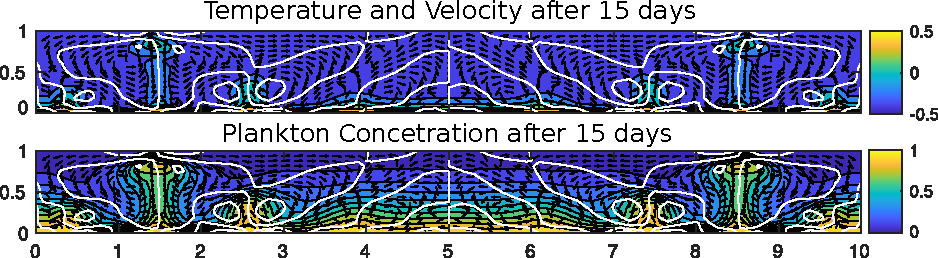
\includegraphics[width=1.0\linewidth]{images/planktonSim.pdf}
\caption{Thermal convection with planktonic mass transfer in the sea.}
\end{figure}

\end{block}


%----------------------------------------------------------------------------------------
%	ACKNOWLEDGEMENTS
%----------------------------------------------------------------------------------------

\setbeamercolor{block alerted title}{fg=black,bg=nyellow} % Change the alert block title colors
\setbeamercolor{block alerted body}{fg=black,bg=white} % Change the alert block body colors
	\vspace{-2em}
\begin{alertblock}{Final Thoughts!}
\textbf{Conclusions}
\begin{itemize}
\item The behavior of the thermal cells depends on the size of the spatial discretization.
\item Even with high Reynolds numbers the implemented method seems to show properlly the general structure of the fluid.
\end{itemize}
\textbf{Pendings}
\begin{itemize}
\item A solver using the projection method was considered, however, the stagered grid was an issue for the energy equation.
\item An implentation using the second order FTBS scheme will help to deal with higher Reynolds numbers.
\end{itemize}

\end{alertblock}
%----------------------------------------------------------------------------------------

\end{column} % End of the third column

\end{columns} % End of all the columns in the poster

\end{frame} % End of the enclosing frame

\end{document}
